\documentclass{article}

% preambuła

% pakiety językowe i formatowanie
%\usepackage[top=2cm, bottom=2cm, left=1cm, right=1cm]{geometry}% marginesy
\usepackage[a4paper]{geometry}
\usepackage[utf8]{inputenc}% kodowanie
\usepackage[T1]{fontenc}% czcionka lepszej jakosci
\usepackage{indentfirst}
\usepackage[polish]{babel}% jezyk polski
\usepackage{polski}

% strona tytułowa
\usepackage{../title}
\subject{Modelowanie i Analiza Systemów Informatycznych}
\subtitle{Logika temporalna i automaty czasowe}
\author{Mykyta Bobrov (224747)\\Paweł Mazur (184197)}
\tutor{dr inż. Paweł Głuchowski}
\group{Pn 9:15}

% odnośniki
\usepackage{url}
%\usepackage{hyperref}
%\hypersetup{colorlinks=true,bookmarks=true,linktocpage}

% wykresy
\usepackage{graphicx}
\usepackage{epstopdf}
\usepackage{pdfpages}
\usepackage{floatrow}

% obramowanie obrazów
\usepackage{float}
%\floatstyle{boxed}
%\restylefloat{figure}

% grafy
\usepackage{tikz}
\usetikzlibrary{arrows,positioning,automata}

% tabele
%\usepackage{slashbox}

% równania
%\usepackage{amsmath}

% listingi
% http://en.wikibooks.org/wiki/LaTeX/Source_Code_Listings
% ftp://ftp.tex.ac.uk/tex-archive/macros/latex/contrib/listings/listings.pdf
\usepackage{listings}
  
% the following is needed for syntax highlighting
\usepackage{color}
   
\definecolor{dkgreen}{rgb}{0,0.6,0}
\definecolor{gray}{rgb}{0.5,0.5,0.5}
\definecolor{mauve}{rgb}{0.58,0,0.82}
  
\lstset{ %
  language=c,
  aboveskip=2em,
  abovecaptionskip=2em,
  %belowcaptionskip=5em,
  %belowskip=3em,
  basicstyle=\footnotesize,       % the size of the fonts that are used for the code
  numbers=left,                   % where to put the line-numbers
  numberstyle=\tiny\color{gray},  % the style that is used for the line-numbers
  stepnumber=1,                   % the step between two line-numbers. If it's 1, each line
                                  % will be numbered
  numbersep=5pt,                  % how far the line-numbers are from the code
  backgroundcolor=\color{white},  % choose the background color. You must add \usepackage{color}
  showspaces=false,               % show spaces adding particular underscores
  showstringspaces=false,         % underline spaces within strings
  showtabs=false,                 % show tabs within strings adding particular underscores
  %frame=single,                   % adds a frame around the code
  rulecolor=\color{black},        % if not set, the frame-color may be changed on line-breaks within not-black text (e.g. commens (green here))
  tabsize=4,                      % sets default tabsize to 2 spaces
  captionpos=b,                   % sets the caption-position to bottom
  breaklines=true,                % sets automatic line breaking
  breakatwhitespace=false,        % sets if automatic breaks should only happen at whitespace
  title=\lstname,                 % show the filename of files included with \lstinputlisting;
                                  % also try caption instead of title
  keywordstyle=\color{blue},      % keyword style
  commentstyle=\color{dkgreen},   % comment style
  stringstyle=\color{mauve},      % string literal style
  escapeinside={\%*}{*)},         % if you want to add a comment within your code
  morekeywords={*}                % if you want to add more keywords to the set
}


\title{Modelowa weryfikacja systemów w~UPPAAL}
\date{8 czerwca 2015}

\begin{document}

	\maketitle
	
	\section{Zadanie 1}
	
		Na potrzeby realizacji pierwszej części zadania został utworzony szablon serwera (\textit{Sever}), klienta (\textit{Client}) oraz sesji (\textit{Session}). Szablony te zostały zaprezentowane kolejno na rys. \ref{figure:server}-\ref{figure:session}.
		
		Klient łączący się do serwera przesyła swój identyfikator (\textit{hs}), który po zatwierdzeniu przez serwer otrzymuje od niego sygnał (\textit{answer}), następnie po podłączeniu (\textit{connected}) tworzona jest sesja klienta (\textit{set\_id}).
		
		Po otwarciu sesji (\textit{Session.Open}) możliwe jest przeście do stanu pobierania (\textit{Session.Download}), który może trwać nie więcej niż 10000 sekund, po czym następuje wylogowanie klienta (przechodzi w stan \textit{Client.Idle}) i zamknięcie sesji (\textit{Session.Closed}).
		
		W przydaku podania przez klienta nieprawidłowego identyfikatora \textit{hs}, połączenie zostaje zablokowane i klient oraz serwer wracją do stanu \textit{Idle} (\textit{Server.Idle}, \textit{Client.Idle}).
		
		\begin{figure}[h]
			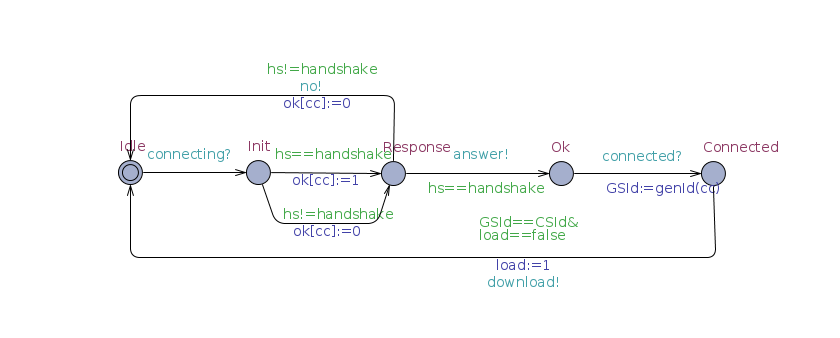
\includegraphics[width=\textwidth]{lab23/server}
			\caption{Szablon serwera}
			\label{figure:server}
		\end{figure}
		
		\begin{figure}[h]
			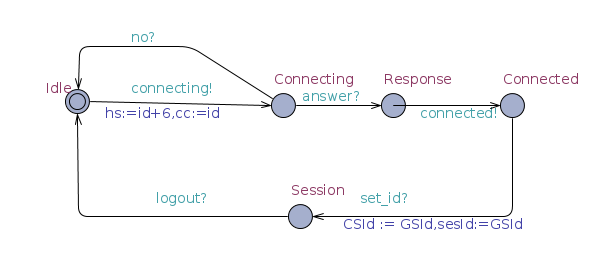
\includegraphics[width=\textwidth]{lab23/client}
			\caption{Szablon klienta}
			\label{figure:client}
		\end{figure}
		
		\begin{figure}[h]
			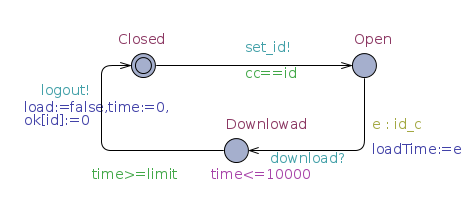
\includegraphics[width=\textwidth]{lab23/session}
			\caption{Szablon sesji}
			\label{figure:session}
		\end{figure}
	
	\newpage
	\section{Zadanie 2}
	
		W celu weryfikacji zbudowanego modelu zostały przygotowane i zweryfikowane następujące własności:
		
		\begin{enumerate}
				
			\item Bezpieczeństwo
			
				\begin{enumerate}
				
					\item Serwer będzie zawsze w stanie oczekiwania (FALSE) \\ $ A[] Server.Idle $
					\item Klienci będą zawsze w stanie oczekiwania (FALSE) \\ $ A[] forall (i:int[0,2]) Client(i).Idle $
				
				\end{enumerate}
			
			\item Osiągalność
			
				\begin{enumerate}

					\item Stan Session procesu Clients napewno będzie osiągnięty (FALSE) \\ $ A<> forall (i:int[0,2]) Client(i).Session $
					\item Stan Session procesu Clients moze zostać osiagnienty (FALSE) \\ $ E<> forall (i:int[0,2]) Client(i).Session $
					\item Klient(2) (majacy poprawny handshake) na pewno otworzy sesje (FALSE) \\ $ A<> Client(2).Session $					
					\item Klient(2) (majacy poprawny handshake) moze otworzyć sesje (TRUE) \\ $ E<> Client(2).Session $
					\item Sesja(2) na pewno zacznie ściągeni (FALSE) \\ $ A<> Session(2).Downlowad $
					\item Sesja(2) może zacząć ściąganie (TRUE) \\ $ E<> Session(2).Downlowad $
					\item Serwer napewno wyśle odpowiedź (FALSE) \\ $ A<>Server.Response $
					\item Serwer może wysłać odpowiedź (TRUE) \\ $ E<>Server.Response $
					\item Serwer na pewno będzie podłączony (FALSE) \\ $ A<> Server.Connected $
					\item Serwer może być podłączony (TRUE) \\ $ E<> Server.Connected $
					\item Sesje na pewno będą zamknięte (TRUE) \\ $ A<> forall (i:int[0,2]) Session(i).Closed $
					\item Sesje moga być zamknięte (TRUE) \\ $ E<> forall (i:int[0,2]) Session(i).Closed $
					\item Serwer na pewno będzie w stanie idle (TRUE) \\ $ A<> Server.Idle $
					\item Server moze być w stanie idle (TRUE) \\ $ E<> Server.Idle $					
					\item Server na pewno będzie w stanie ok (FALSE) \\ $ A<> Server.Ok $
					\item Server może być w stanie ok (TRUE) \\ $ E<> Server.Ok  $					
				
				\end{enumerate}
				
			\item
				
				\begin{enumerate}
				
					\item Jeśli sesja będzie zamknieta to ściągenie pliku sie skończy (TRUE) \\ $ forall (i:int[0,2]) Session(i).Closed --> load==false $
					\item Jeśli ktoś ściąga plik to ściąganie jest możliwe (FALSE) \\ $ load!=true --> forall (i:int[0,2]) Session(i).Downlowad $
				
				\end{enumerate}
			
		\end{enumerate}
		
		\begin{figure}[h]
			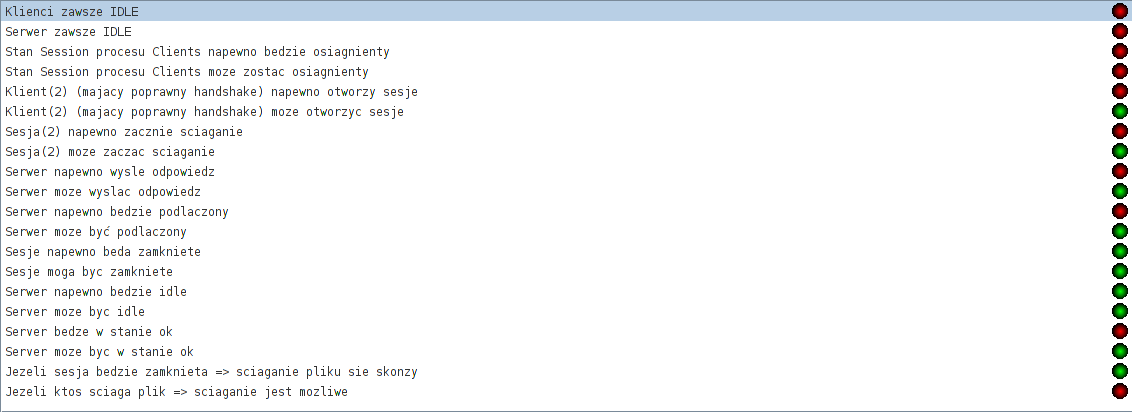
\includegraphics[width=\textwidth,angle=90]{lab23/verifier}
			\caption{Wynik działania weryfikatora w progremie UPPALL}
		\end{figure}
		
			
\end{document}
